\documentclass[10pt]{article}
\usepackage[table]{xcolor}  % load xcolor before anything else
\usepackage[most]{tcolorbox}
\usepackage{setspace}  %line spacing
\usepackage{titling}
\usepackage{graphicx}
\usepackage{parskip}    %spaced paragraphs
\usepackage{csquotes}   %babel wanted it
% \usepackage{emptypage} % prevent page numbers and headings on empty pages
\usepackage{float} % for H specification
% \usepackage{censor}
\usepackage{amsmath}
\usepackage{fontawesome}    % fancy font special characters
% \usepackage{pdfpages} % insert pdf 
\usepackage[titletoc]{appendix}
\usepackage{pdflscape} % landscape pdf pages
\usepackage{wrapfig}
\usepackage{booktabs,nicematrix} % quality tables 

% \usepackage{tikz}
% \usepackage{circuitikz}
% \usetikzlibrary{calc}
% \usetikzlibrary{arrows,positioning}
% \usetikzlibrary{graphs, graphs.standard}

\usepackage[hang,flushmargin]{footmisc}     % footnote editing

\usepackage[font=small,labelfont=bf,justification=centering]{caption} % caption size 
\usepackage{subcaption}
\setlength{\belowcaptionskip}{-5pt}

\usepackage[hidelinks]{hyperref}  %have a review of this
\hypersetup{%
%   citecolor=black,
  colorlinks=false,
%   linkcolor=black,
%   urlcolor=black
}
\usepackage[nameinlink]{cleveref}

\usepackage{listings}% code
\definecolor{codegreen}{rgb}{0,0.6,0}
\definecolor{codegrey}{rgb}{0.5,0.5,0.5}
\definecolor{codepurple}{rgb}{0.58,0,0.82}
\definecolor{backcolour}{rgb}{0.95,0.95,0.92}
\lstdefinestyle{codestyle}{
    backgroundcolor=\color{backcolour},   
    commentstyle=\color{codegrey},
    keywordstyle=\color{blue},
    numberstyle=\tiny\color{codegrey},  % line numbers
    stringstyle=\color{codegreen},
    basicstyle=\ttfamily\lst@ifdisplaystyle\footnotesize\fi,
    breakatwhitespace=false,         % sets if automatic breaks should only happen at whitespace
    breaklines=true,                 % sets automatic line breaking
    captionpos=t,                    
    keepspaces=true,                 % keeps spaces in text, useful for keeping indentation of code (possibly needs columns=flexible)
    numbers=left,
    stepnumber=1,                    % the step between two line-numbers. If it's 1, each line will be numbered                    
    numbersep=5pt,                   % how far the line-numbers are from the code
    showspaces=false,                % show spaces everywhere adding particular underscores; it overrides 'showstringspaces'
    showstringspaces=false,          % underline spaces within strings only
    showtabs=false,                  % show tabs within strings adding particular underscores
    % tabsize=2,                       % sets default tabsize to 2 spaces
    framextopmargin=50pt,
    % title=\lstname,                  % show the filename of files included with \lstinputlisting; also try caption instead of title
    columns=fixed,                   % Using fixed column width (for e.g. nice alignment)
    frame=bottomline,
    % frame=tb,
    % belowcaptionskip=0pt,
    aboveskip=3pt,
    belowskip=3pt,
    % texcl=true,
}
\lstset{style=codestyle}

\usepackage{geometry}
\geometry{a4paper, margin=1.5cm}

\usepackage{fontspec}
\setmainfont[ 
    Mapping=tex-text,
    BoldFont={HelveticaNowText-Bold},
    ItalicFont={HelveticaNowText-RegIta},
    BoldItalicFont={HelveticaNowText-BoldItalic}
]{[HelveticaNowText-Regular]}
\usepackage{sansmath}
\sansmath

\usepackage{fancyhdr}   %footer
\fancypagestyle{myheadings}{%
    \fancyhf{}
    \renewcommand{\headrulewidth}{0.5pt}
    \renewcommand{\footrulewidth}{0pt}
    \addtolength{\headheight}{2pt}
    % \fancyhead[L]{\leftmark}
    \fancyhead[L]{ES3B2: Digital Systems Design}
    \fancyhead[R]{1922268}
    \cfoot{\thepage}
}
\pagestyle{myheadings}

\usepackage{enumitem}   %reduce list spacing
\setlist{nosep} 

\usepackage[
    backend=biber,
    style=numeric-comp,
    % style = vancouver,
    % style = science,
    % style=draft,
    % style = ieee,
    % maxnames=2, minnames=2,
    % doi=false,
    sorting=none
]{biblatex}   %bibliography
\usepackage{xurl} % break urls. load after biblatex
\addbibresource{sections/refs.bib}

\usepackage[
    separate-uncertainty=true,
    multi-part-units=single
    ]{siunitx}
\sisetup{
    detect-all,
    per-mode=symbol-or-fraction,
    tight-spacing,
    % quantity-product =,
    number-unit-product=\,,
    % space-before-unit=true
}
\DeclareSIUnit{\mAh}{mAh}

\usepackage{xltabular}
\usepackage{multirow}
\newcolumntype{Y}{>{\centering\arraybackslash}X}
\newcolumntype{Z}{>{\raggedright\arraybackslash}X}
\newcolumntype{P}[1]{>{\centering\arraybackslash}p{#1}}

\newenvironment{conditions}[1][where:]
  {#1 \begin{tabular}[t]{>{$}l<{$} @{} >{${}}c<{{}$} @{} l}}
  {\end{tabular}\\[\belowdisplayskip]}

\definecolor{titlepagecolour}{HTML}{003D99}
\definecolor{titleblue}{HTML}{1b1787} % blue
\definecolor{tableh1}{HTML}{dae3eb} %table grey
\definecolor{tableh2}{HTML}{b3ccf5} %table bluegrey
\definecolor{tableg}{HTML}{309c3d} % green
\definecolor{tablea}{HTML}{ed901f} % amber
\definecolor{tabler}{HTML}{f2422e} % red

\definecolor{hCyan}{HTML}{00FFFF}
\definecolor{hMagenta}{HTML}{FF00FF}
\definecolor{hBlue}{HTML}{0000FF}

\usepackage[british]{babel} 

% \usepackage{pgfgantt}
% \setganttlinklabel{s-s}{}
% \setganttlinklabel{f-s}{}
% \setganttlinklabel{f-f}{}

% \usepackage{titlesec} 
% \titlespacing\section{0pt}{12pt plus 4pt minus 2pt}{0pt plus 2pt minus 2pt}
% \titlespacing\subsection{0pt}{12pt plus 4pt minus 2pt}{0pt plus 2pt minus 2pt}
% \titlespacing\subsubsection{0pt}{12pt plus 4pt minus 2pt}{0pt plus 2pt minus 2pt}
% \titlespacing\paragraph{0pt}{10pt plus 4pt minus 2pt}{10pt plus 2pt minus 2pt}

\begin{document}
% \onehalfspacing
% \setstretch{1.25} % one and quarter spacing

\section{Introduction to VGA}\label{sec:intro}
VGA (Video Graphics Array) is a visual graphics standard introduced in 1987.
It was developed to work with CRT (Cathode-Ray Tube) technology, which works 
by drawing each pixel in horizontal lines vertically down the display to 
create a \emph{frame}.

In order to produce the effect of a static image 
given only a single pixel controlled per instant, the entire frame 
would be redrawn (or `refreshed') quicker than the eye can perceive.
A refresh rate of \qty{60}{\Hz} would be typical.

Due to the physical deflection of an electron beam to produce pixels, 
extra time for the beam to adjust to a new line is included in the standard, called 
the \emph{blanking interval}. 
The start of a new line is controlled by the horizontal sync (hsync) signal, with a 
new frame in turn controlled by a vertical sync (vsync) signal. The blanking intervals before 
and after these signals are respectively called the \emph{front porch} and \emph{back porch}. 
In modern standards like HDMI, this extra time has been retained and instead carries extra 
data like accompanying audio. 


\subsection{Driving the display}\label{sec:drivingdisplay}

There are four requirements for driving a VGA display:
\begin{enumerate}
    \item Clock signal driving the display signal counters.
    \item Horizontal and vertical signals, defining pixels.
    \item Drawing graphical elements to the screen.
    \item Physical video output to a display.
\end{enumerate}

\subsubsection{Clock}
The required display frequency clock can be calculated by:
\begin{align*}
    f_{\text{clock}} & = L_h \times L_v \times f_{r}
\end{align*}

\begin{conditions}
    L_h & = & horizontal lines, 1903 \\
    L_v & = & vertical lines, 931 \\
    f_{r} & = & refresh frequency, \qty{60}{\Hz} \\
\end{conditions}

% where: 
% \begin{tabular}[H]{ l c l}
%     $\lambda$ & $=$ & wavelength \\
%     $v$ & $=$ & velocity, which in this case will be $c$, the speed of light \\
%     $f$ & $=$ & frequency \\
% \end{tabular}\\

The results in a required clock frequency of \qty{106.30158}{\MHz}. 
The easiest method of producing clock signals in Verilog is to divide down the main 
processor clock to the required subdivision. In the case of the 
Nexys A7, the onboard clock is \qty{100}{\MHz} and thus cannot be divided down to 
a value that is greater. However, by using the Clocking Wizard IP provided by Xilinx, 
this can be produced. The caveat is that it will not be necessarily exact. 
In this case, the actual output clock is \qty{106.296}{\MHz}, which is within \qty{0.005}{\percent}.

\subsubsection{Signals}
In this implementation, the horizontal and vertical signals are controlled by counters 
operating at the overall display frequency, determining which pixel is being drawn. 
The counter values then determine the widths of each signal parameter.
The parameters are outlined in \cref{table:vgaparams}, which informs the display dimensions
as shown in \cref{fig:vga}.
\begin{xltabular}{\linewidth}{Y|YYYY}
    & Sync signal & Back porch & Display & Front porch \\
    \hline
    Horizontal & 151 & 384 & 1824 & 1903 \\
    \hline
    Vertical & 2 & 30 & 930 & 931 \\
    \hline
    \caption{VGA signal parameters}\label{table:vgaparams}
\end{xltabular}
The visible portion produces a display resolution of 1440x900. 

\begin{figure}[htbp]
    \centering
    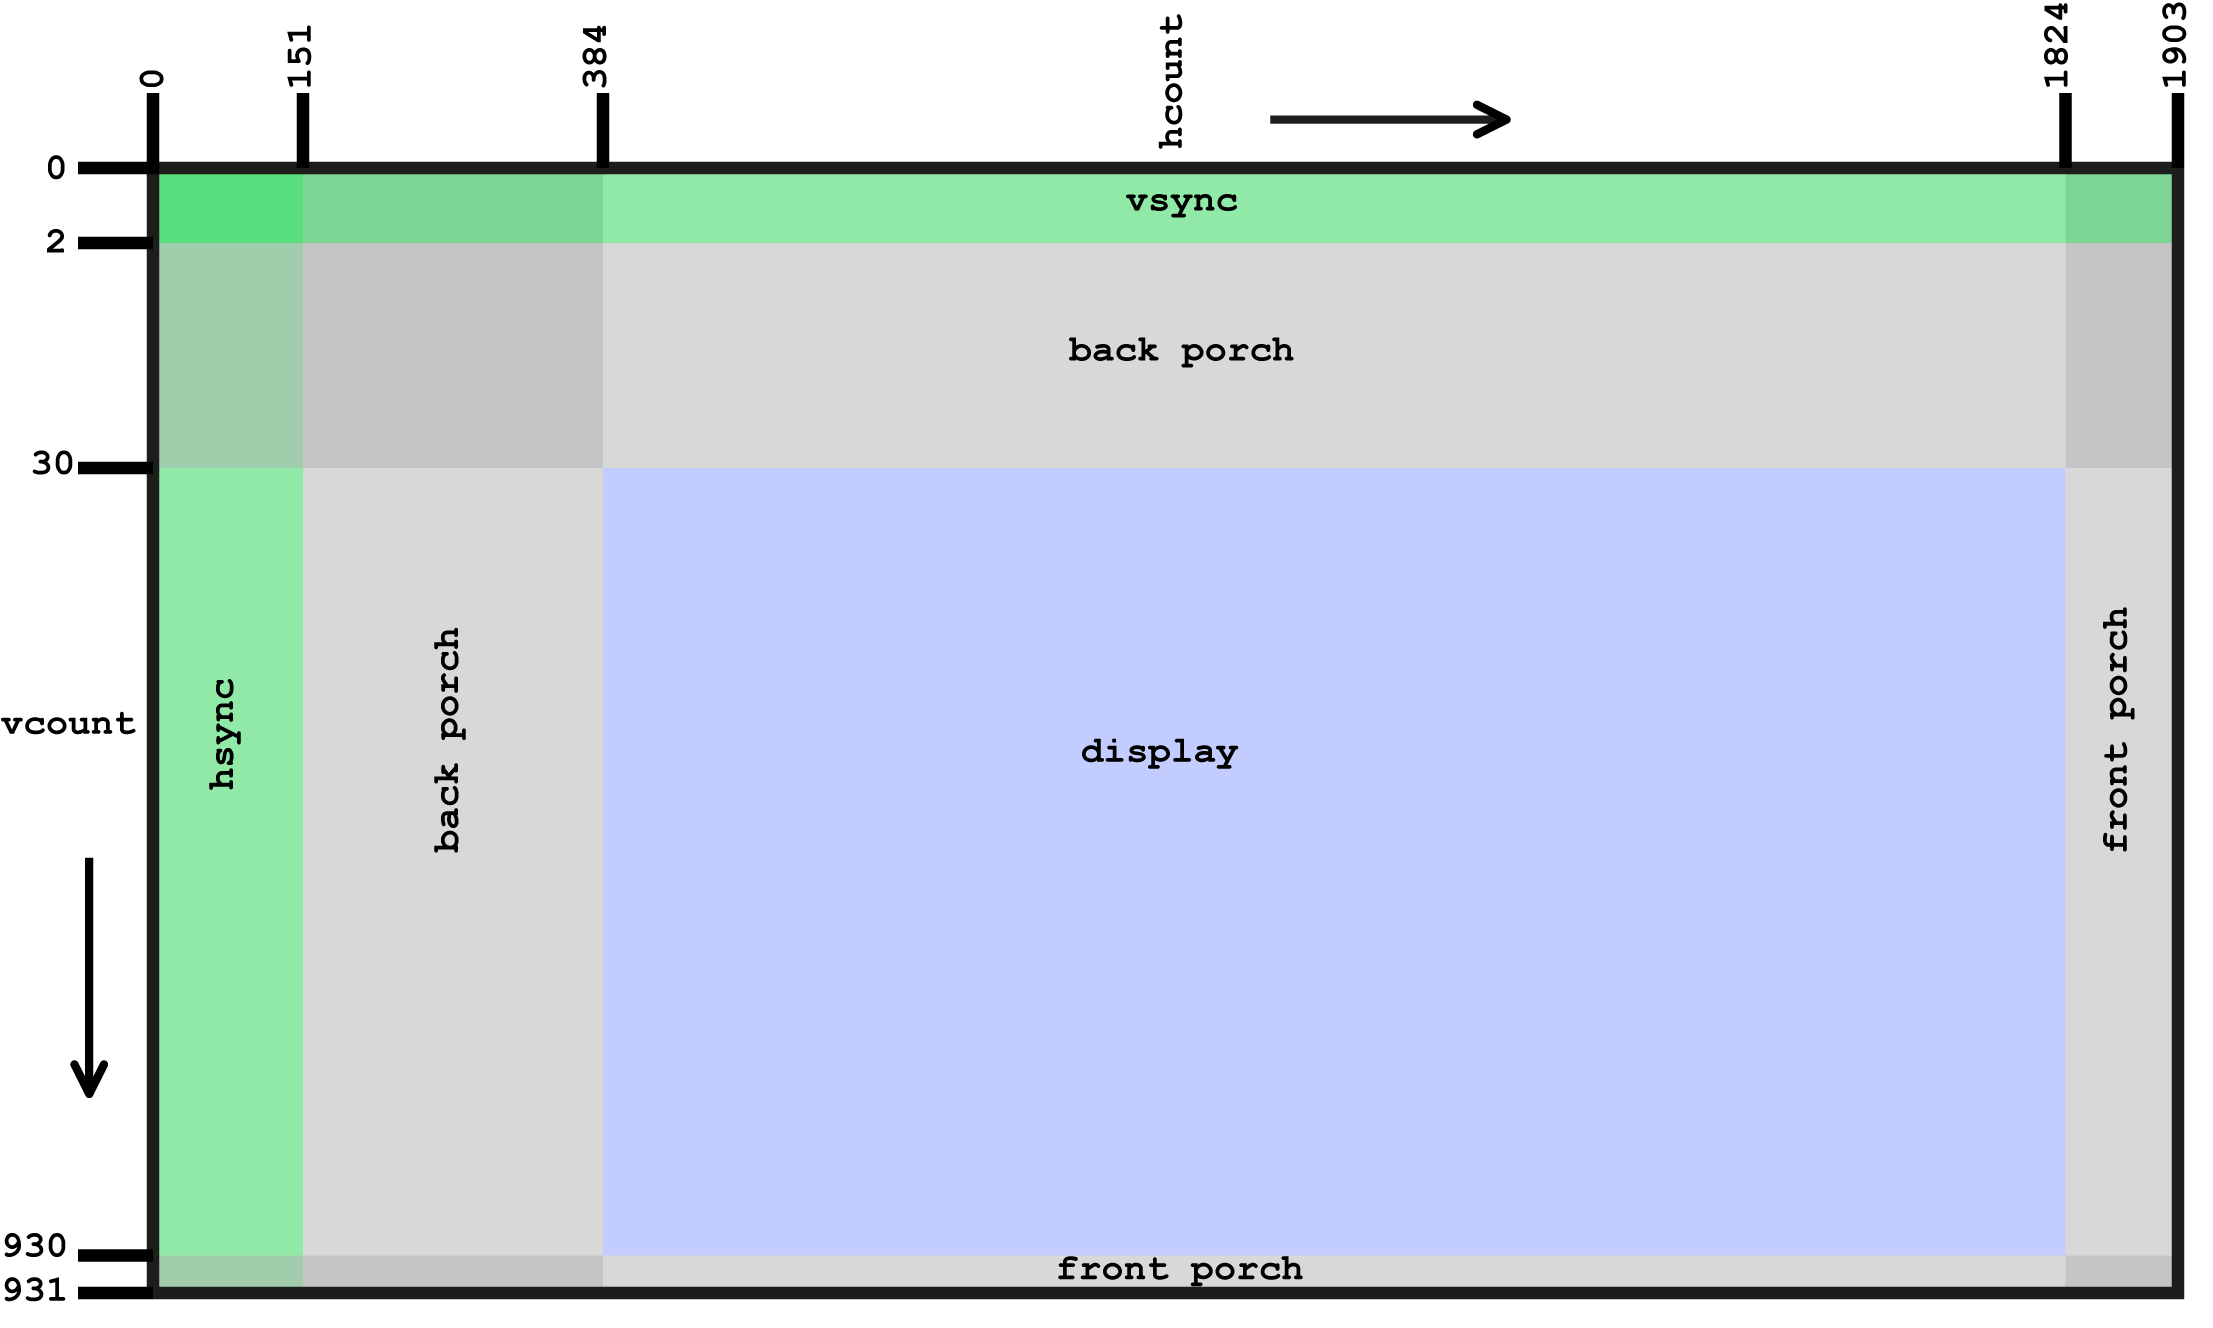
\includegraphics[width=0.8\textwidth]{./figures/vga display.png}
    \caption{Display parameters}\label{fig:vga}
\end{figure}

\subsubsection{Drawing graphics}
Graphics drawing is delegated to its own module\footnote{
    \Cref{sec:drawcon}.
} separate from the VGA controller. 
To provide an overview, the graphics drawing module (draw controller) takes as input the 
current pixel by coordinates in \emph{x} and \emph{y} with reference to the top left corner
of the visible display. It outputs the colour for this pixel as a 12-bit hexadecimal number, which can then 
be passed to the VGA port.

\subsubsection{Video output}
The specifics of the output (i.e. required voltages, pin connections etc. to the D-sub connector) is
abstracted away in the constraints file for the board. In this file, the pins of the Nexys A7 
with regard to the VGA port are provided and simply need to be 
included in the compilation to be used. 

The colour channels in the port are different physical connections, taking up six pins of the 
connector - one each for red, green, and blue, in addition to each colour's ground reference. 
In the implementation for this project, the 4-bit output colour variables
(\lstinline{VGA_R}, \lstinline{VGA_G}, \lstinline{VGA_B}) 
have been merged into a single 12-bit variable (\lstinline{colour}). 

The mapping occurs as follows:

\begin{tabular}{l|lll}
    Original & \lstinline|VGA_R[3:0]| & \lstinline|VGA_G[3:0]| & \lstinline|VGA_B[3:0]| \\
    Implementation & \lstinline|colour[11:8]| & \lstinline|colour[7:4]| & \lstinline|colour[3:0]| 
\end{tabular}
% \begin{lstlisting}[numbers=none,frame=none]
%         Original        |    VGA_R[3:0]     VGA_G[3:0]      VGA_B[3:0]
%         Implementation  |    colour[11:8]   colour[7:4]     colour[3:0] 
% \end{lstlisting}

The advantage of this is that colour assignment to a pixel can now be encoded as a single hexadecimal number 
with three digits - the first encoding the red value, the second green, and the third blue. 
This is particularly useful as the encoding now follows web-safe hexadecimal colour space\footnote{
    A palette reference available at \href{https://www.rapidtables.com/web/color/Web_Safe.html}{RapidTables \faExternalLink}.
}, reducing the guesswork in developing a colour on screen.

\subsection{Limitations}
With VGA as the only display adapter available on the board, the colours available is limited 
to 4-bits for the red, green, and blue channels each. This results in 4096 total colours. 
Most modern monitor displays, on the other hand, permit over 16 million colours due to the 
use of 24-bit colour space. 

\subsection{Implementation}
The implementation of the VGA controller can be found in \cref{code:vga}.

\section{The game}
\subsection{Gameplay}
The player controls a reticle in a bounded box with a colour gradient, which is placed on a grid of colours.
The player selects a colour within the gradient 
by tilting the board until the reticle is positioned above the colour to be selected.
The aim is to select colours in 
order to clear the grid as quickly as possible. When a cell in the grid is selected (`matched'), it 
follows the reticle in its colour selection. As more colours are selected, a greater portion of the screen is matched 
until the background is a solid colour. To begin with, only the cells surrounding the central selector can be matched,
however colours can then be matched to any successive cells that have also been matched, `flooding' from the central region. 
\begin{figure}[ht]
    \centering
    \begin{subfigure}[t]{0.3\linewidth}
        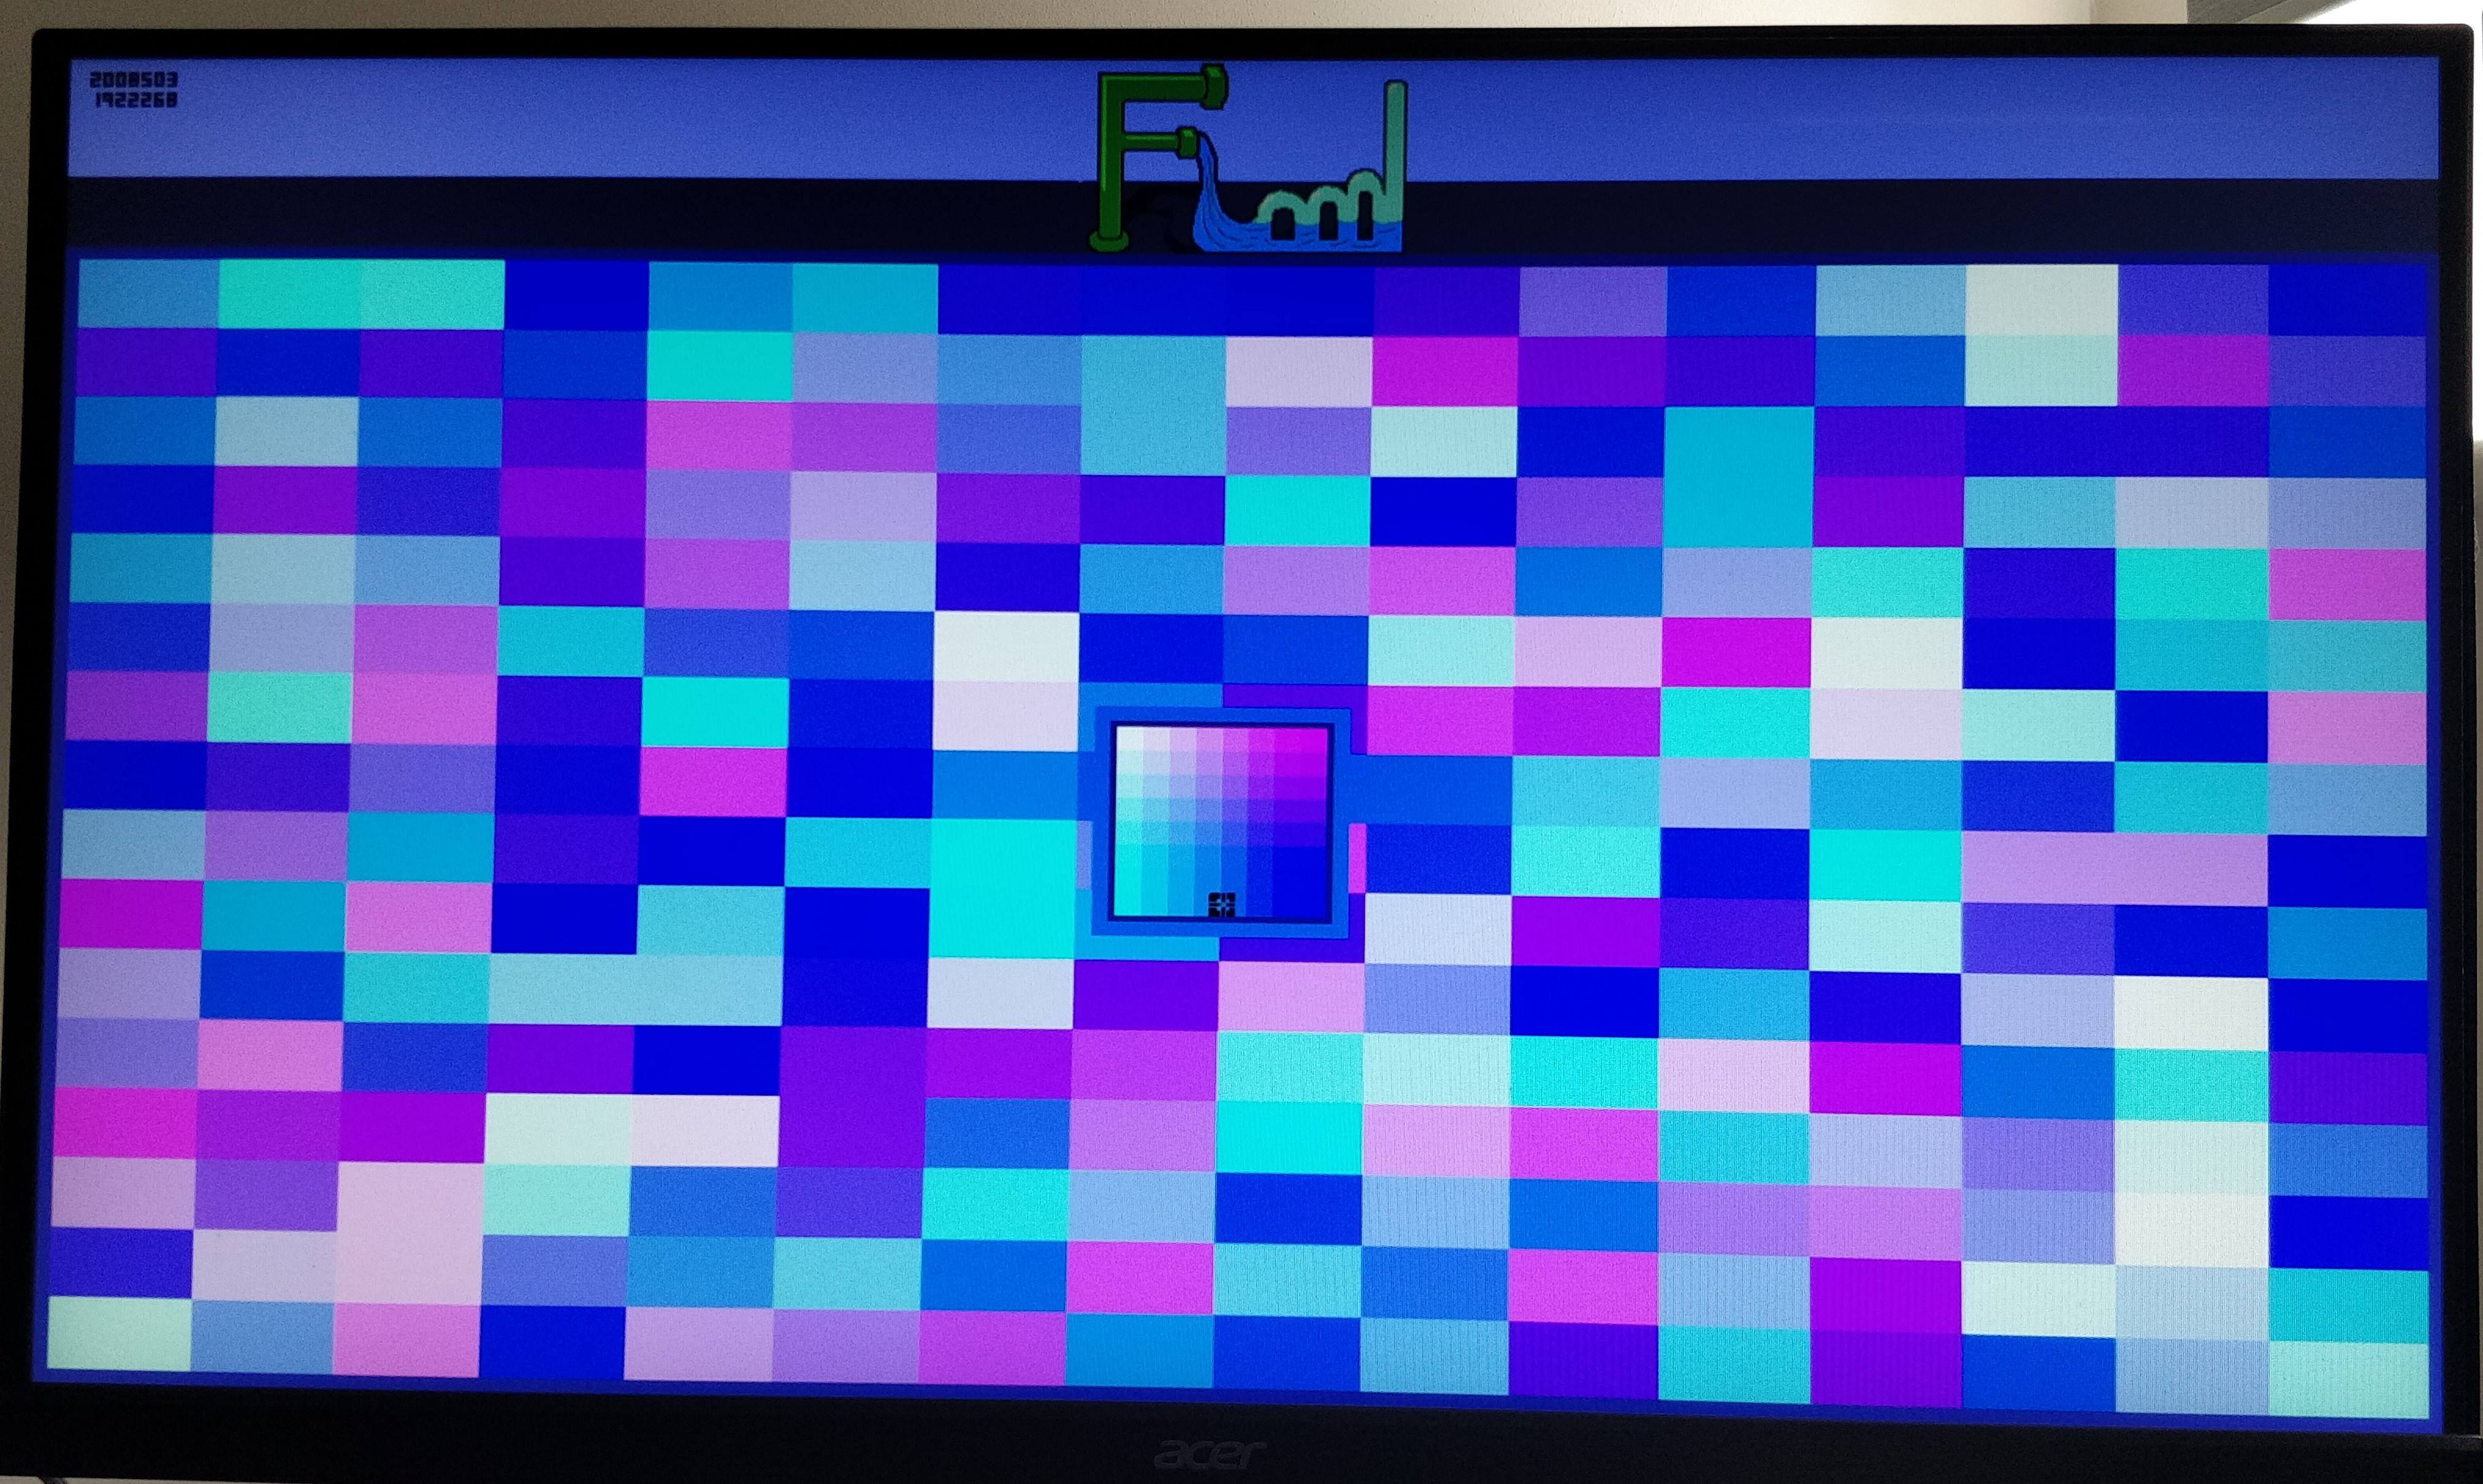
\includegraphics[width=\linewidth]{figures/start-1.jpg}
        \caption{Start}
    \end{subfigure}
    \hfill    
    \begin{subfigure}[t]{0.3\linewidth}
        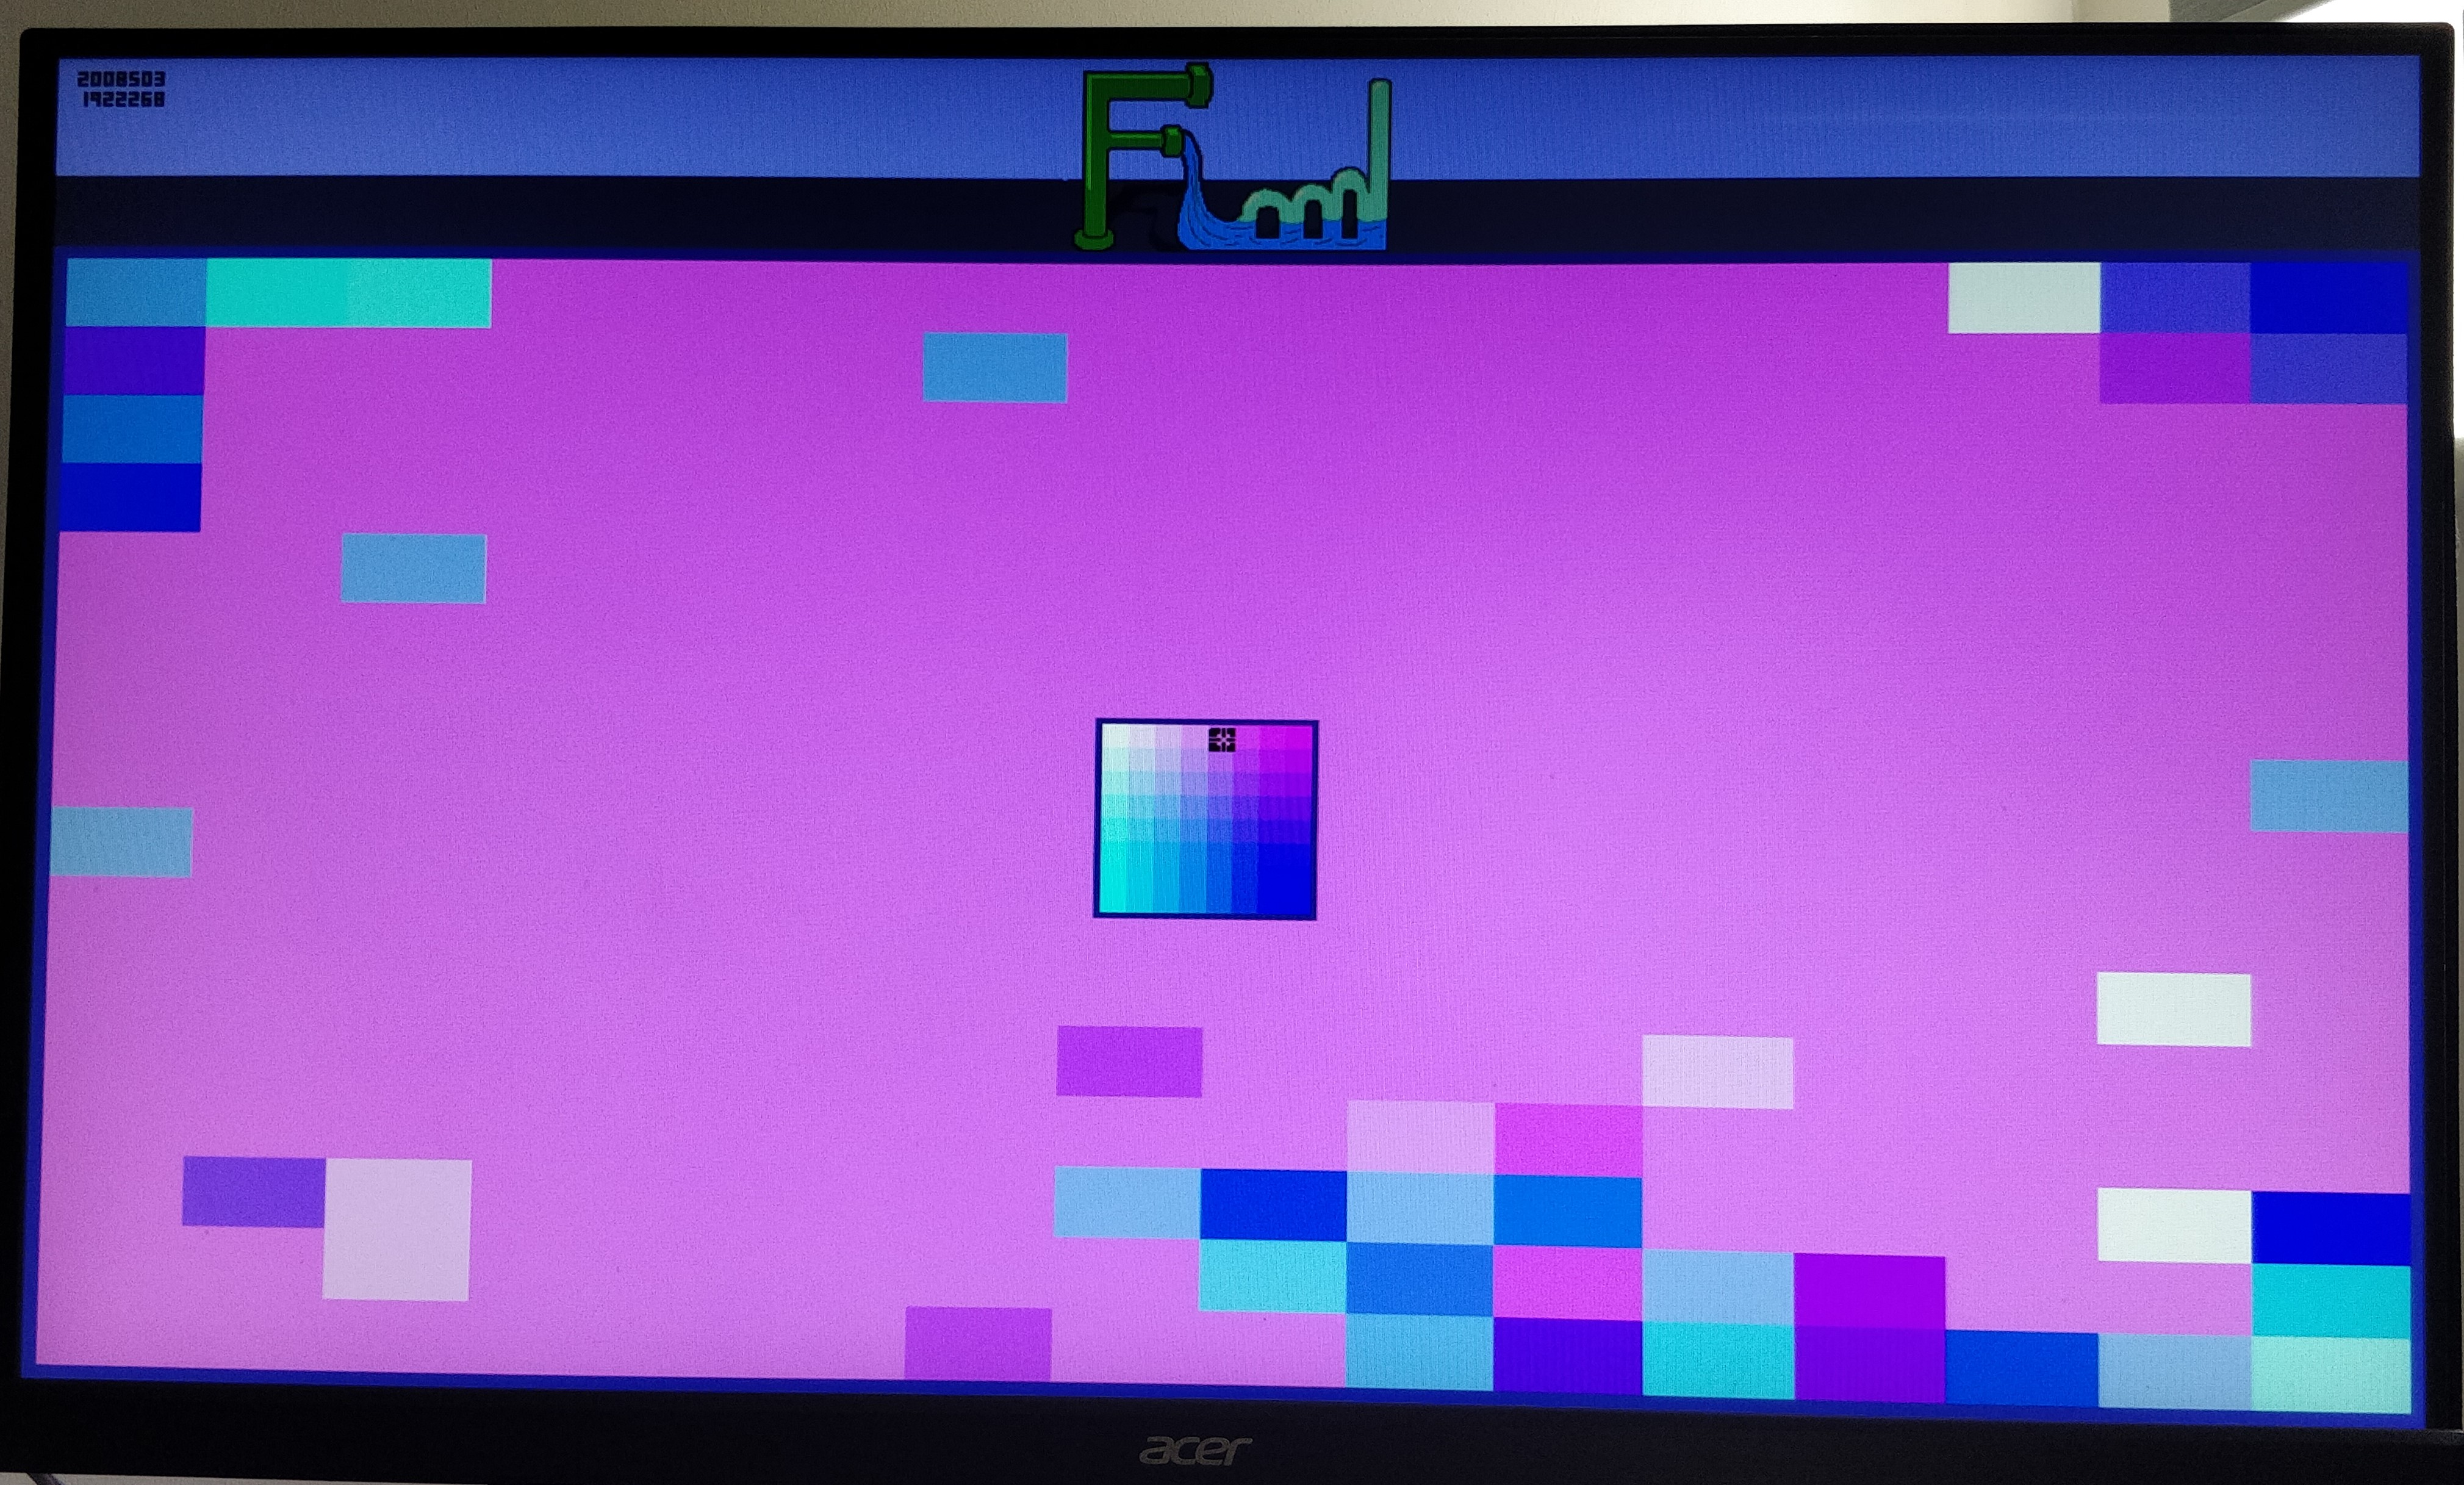
\includegraphics[width=\linewidth]{figures/partway-1.jpg}
        \caption{Partway}
    \end{subfigure}
    \hfill    
    \begin{subfigure}[t]{0.3\linewidth}
        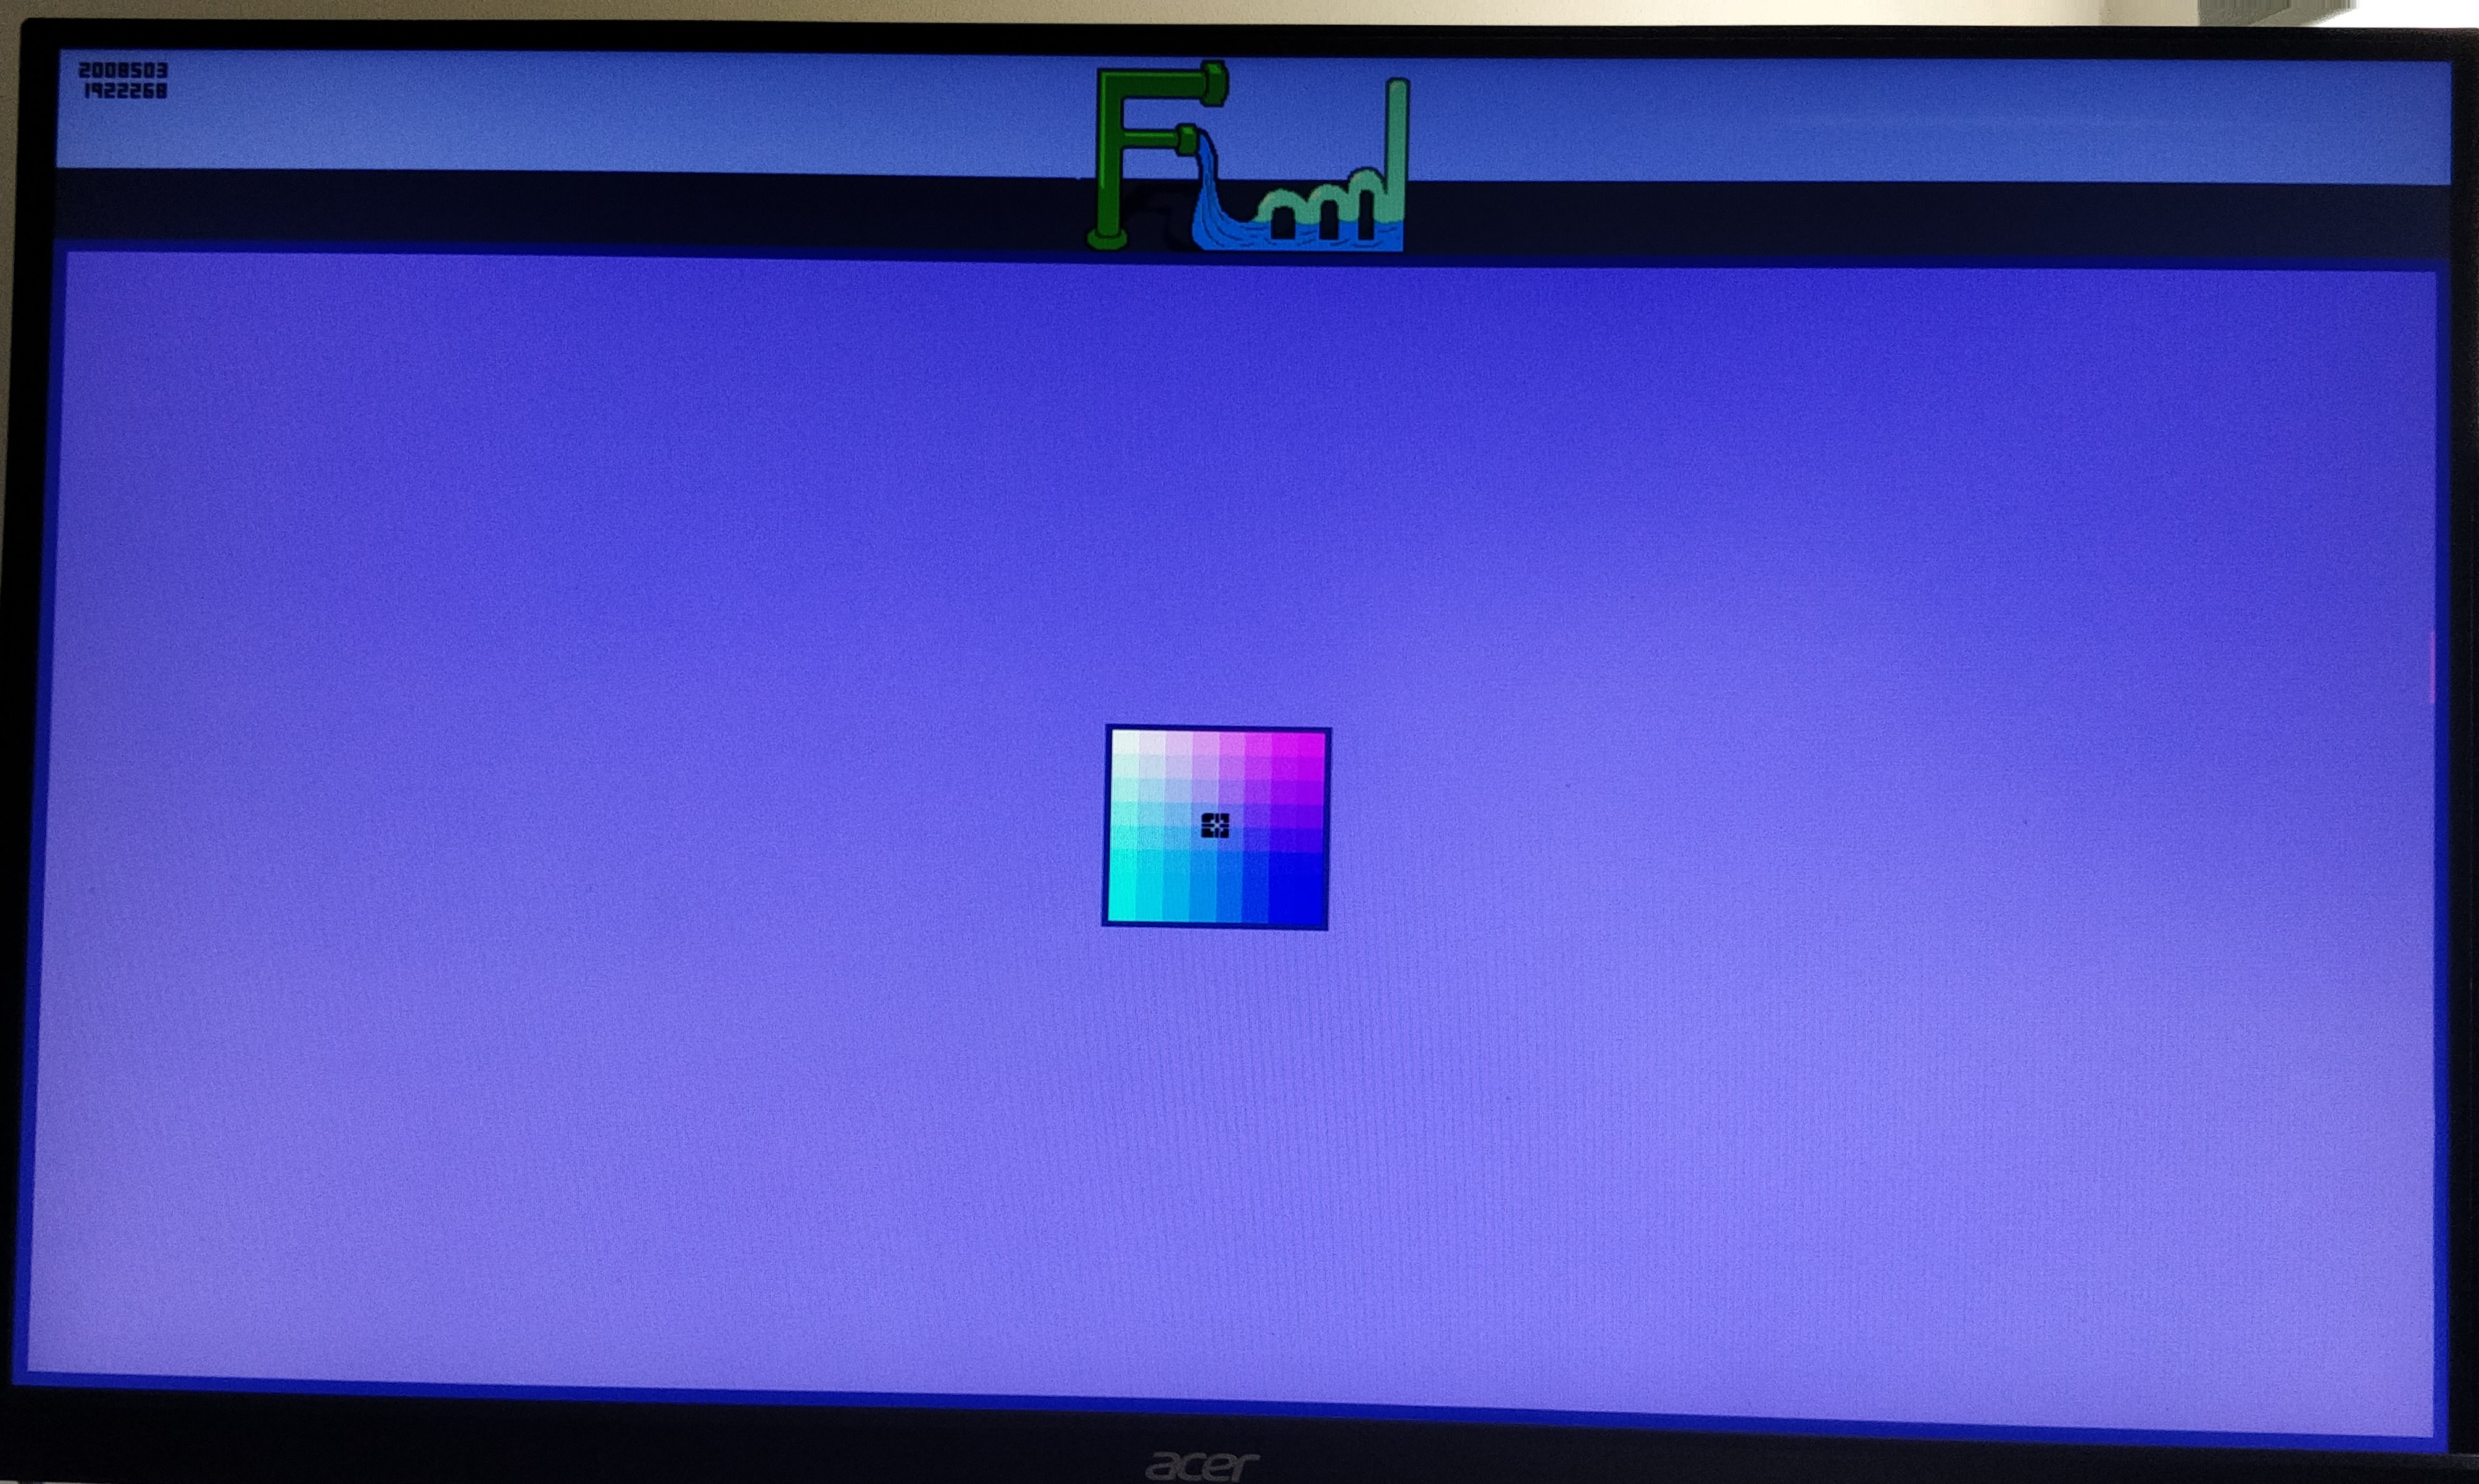
\includegraphics[width=\linewidth]{figures/complete-1.jpg}
        \caption{Cleared!}
    \end{subfigure}
    \caption{Gameplay states}
\end{figure}
\subsection{Module overview}
The structure of the program follows a hierarchical design, with module \lstinline{game_top} as the 
parent module. The relationships and data connections between modules is demonstrated in \cref{fig:relationship}. 
This module specifies many parameters that are carried over to child modules.
\begin{figure}[H]
    \centering
    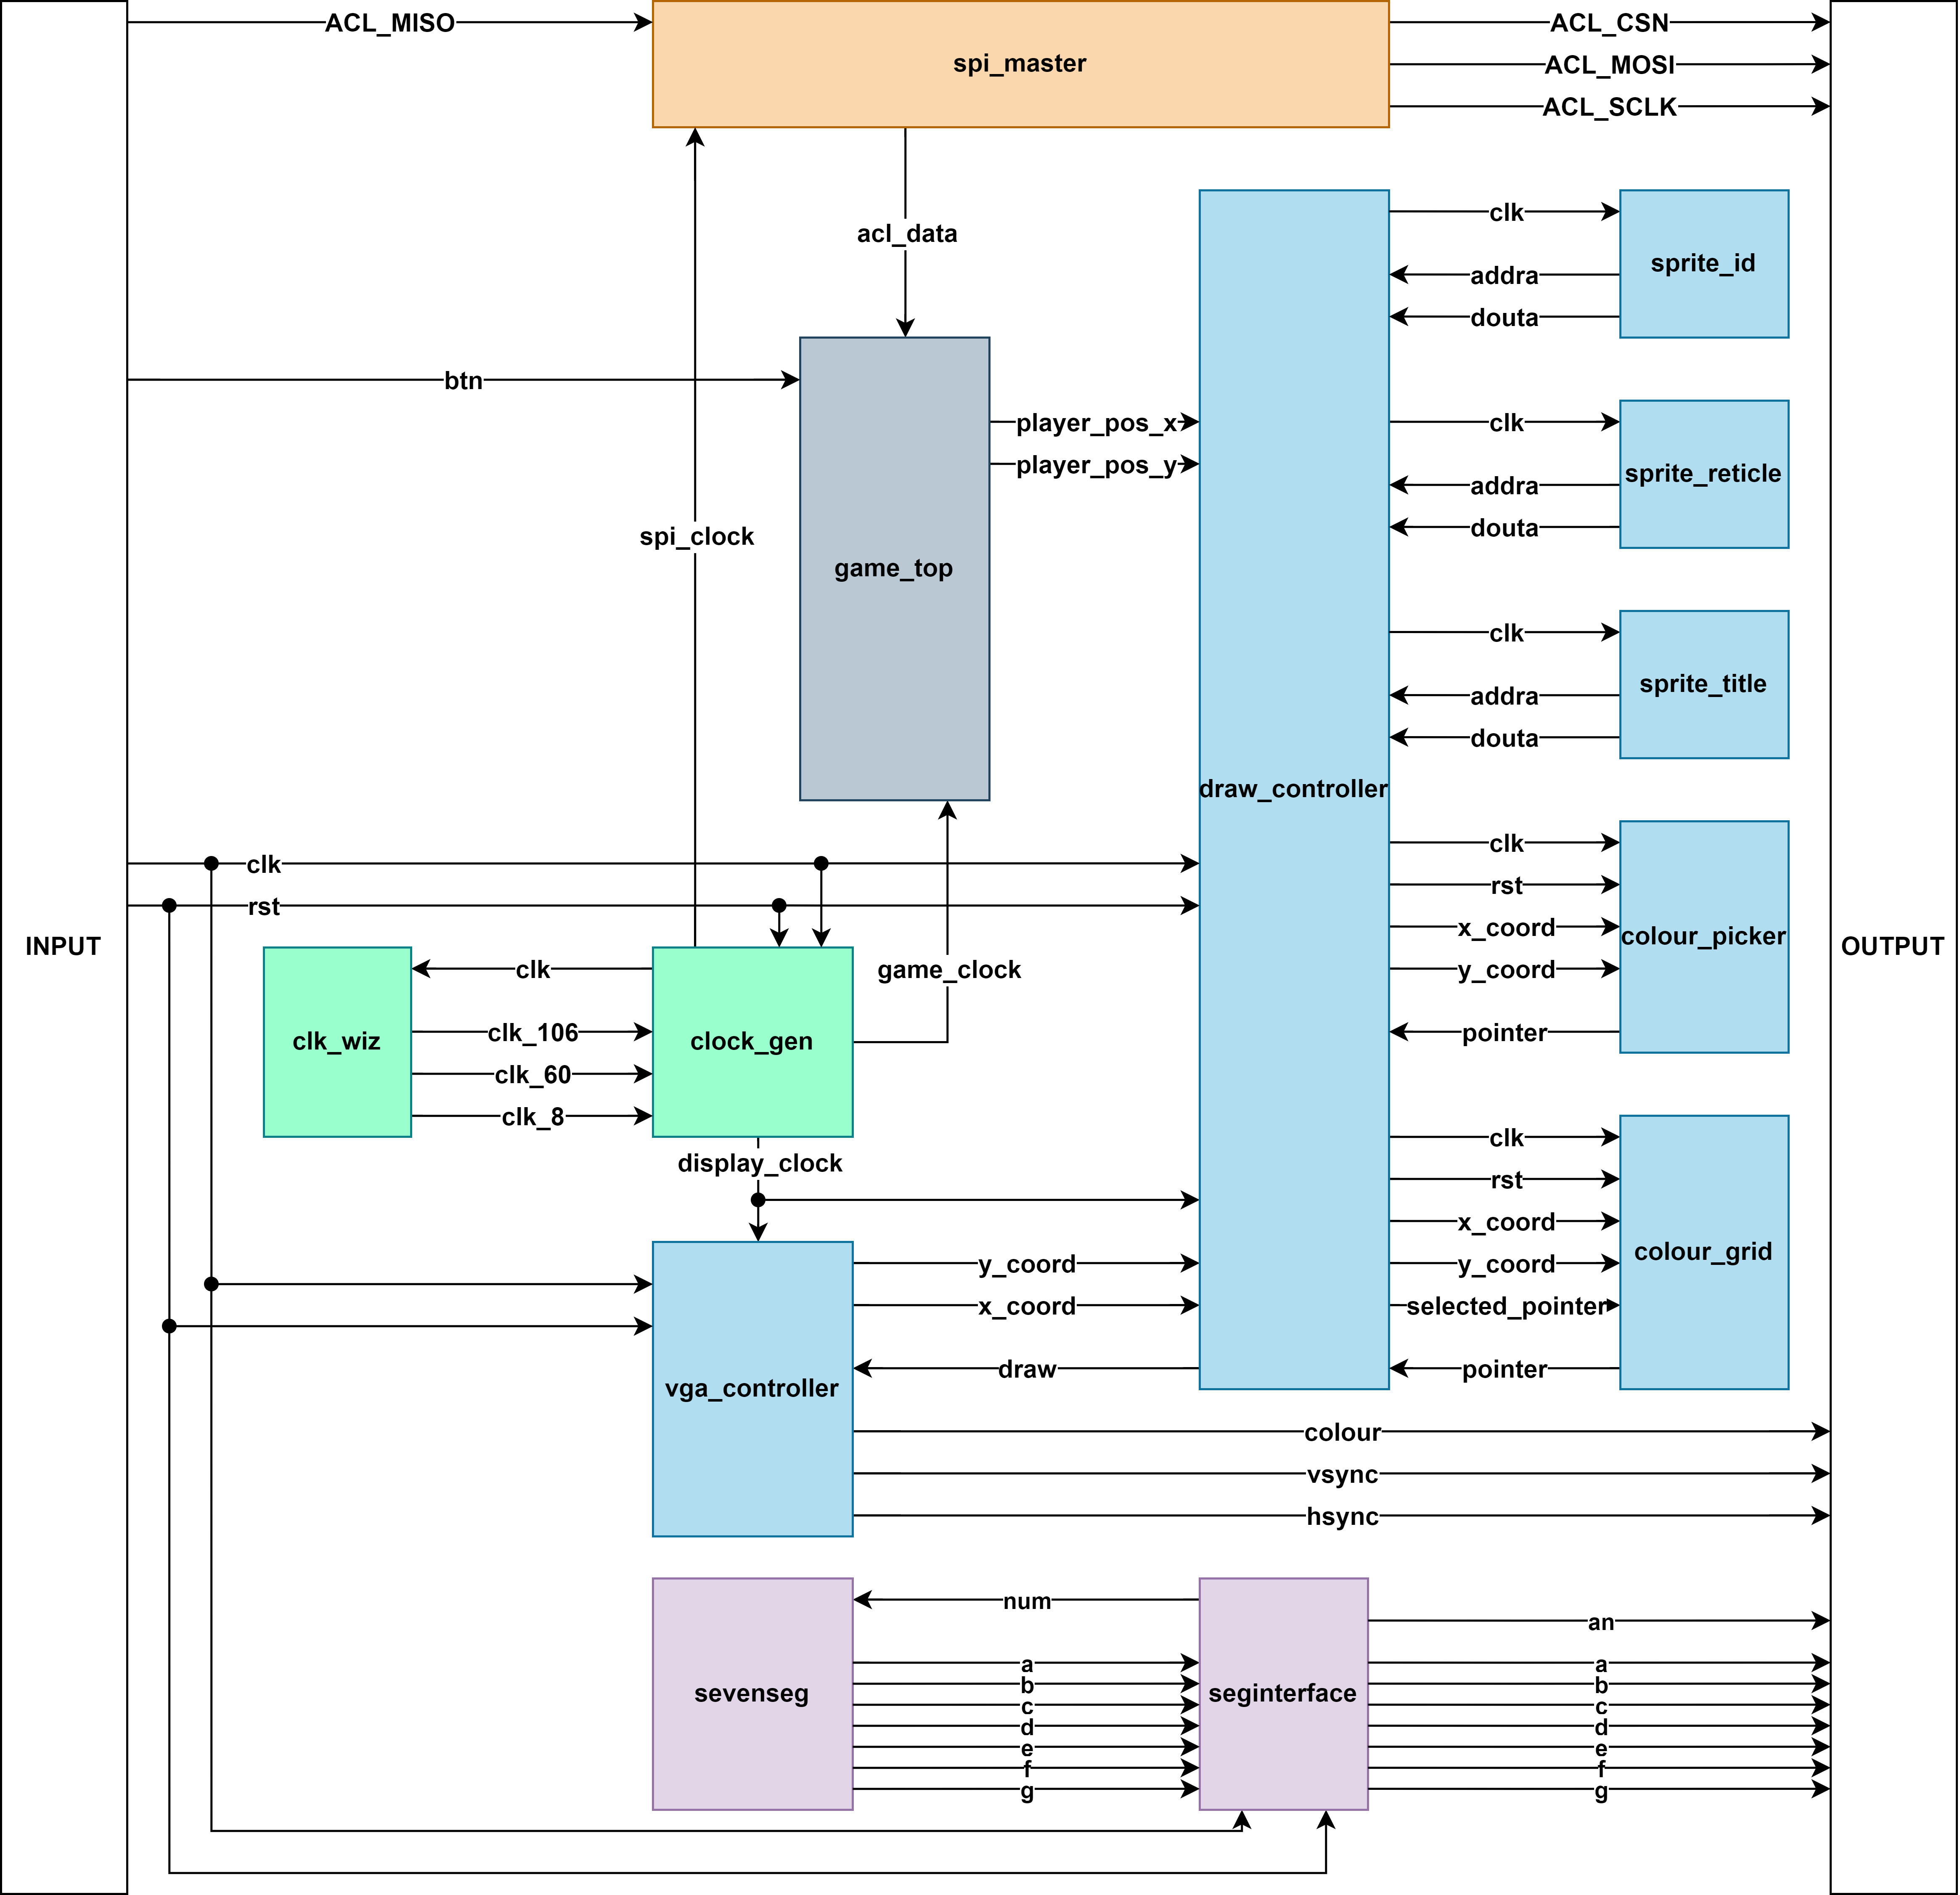
\includegraphics[width=\textwidth,height=0.5\textheight,keepaspectratio]{./figures/relationship.png}
    \caption{Relationship diagram}\label{fig:relationship}
\end{figure}
The following sections discuss the constituent modules in detail. 

\subsection{game\_top}\label{sec:gametop}
Code available in \cref{code:gametop}.

This module is the topmost module, and primarily handles connections both to the board's peripherals 
from modules, and between modules themselves. It additionally controls movement logic for the 
player sprite\footnote{
    \Cref{sec:sprite}.
}.

\begin{wrapfigure}[7]{R}{0.35\textwidth}
    \vspace{-11pt}
    \begin{center}
        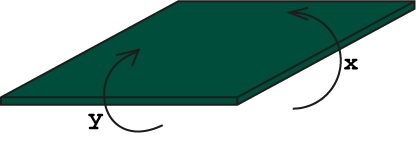
\includegraphics[width=0.32\textwidth]{figures/boardtilt.png}
        \caption{Accelerometer tilt influence}\label{fig:acltilt}
    \end{center}
\end{wrapfigure}

The accelerometer controller\footnote{
    \Cref{sec:spi}.
} outputs a single 15-bit string of data, \lstinline|acl_data|, encoding five bits of \emph{x}, \emph{y},
and \emph{z} orientation data each. For the purposes of this project, only the \emph{x} and \emph{y} 
data are needed, with the tilt directions indicated in \cref{fig:acltilt}. The relevant data can 
be accessed with a bit-slice \lstinline|acl_data[9:5]| for \emph{x} and \lstinline|acl_data[14:10]|
for \emph{y}. 

The 5-bits of returned data indicates the level of tilt, with 0 meaning level, 15 meaning a \qty{90}{\degree}
rotation anticlockwise/left in \emph{x} and clockwise/forward in \emph{y}, and 31 meaning an almost complete rotation.
In order to adapt this to control movement, these values need to be split and adjusted. 
Regarding horizontal movement of the player sprite, a value of 0-15 can be added to \lstinline{player_pos_x} 
to update position, producing a translation to the right. A negative value produces a translation left. 
Tilting the board left returns 0-15, so this simply needs to be negated from the player position to produce
the desired translation. Tilting the board right returns 31-16, so first a subtraction from 31 is performed,
and then the value is added to position\footnote{
    Lines 55-70.
}. 

In order to bound the player movement, so it does not move out of the colour selection area, two changes are needed. 
First, the bounding parameters, i.e. the maximum and minimum coordinates the player can move to, can be specified 
in parameters. Then, each time the player position is to update, the current position in addition to the updated position 
is compared to the bounding parameter. If greater, the current position is set to the bounding parameter\footnote{
    Lines 72-88.
}.  
This maintains a smooth collision with the bounding walls. 


\subsection{spi\_master}\label{sec:spi}
This module is used to communicate with the ADXL362 \cite{adxl362} accelerometer, which is exposed on the 
SPI interface. The code in this module is written by David Marion as part of his 
experimentation with FPGAs and is available on his GitHub \cite{fpgadudeacl}.

The module collects data from the accelerometer and returns a 15-bit number encoding \emph{x}, \emph{y}, and \emph{z} 
acceleration data, which has been adapted in \lstinline{game_top}\footnote{
    \Cref{sec:gametop}.
} to produce movement of the player sprite. 

\subsection{clock\_gen}
Code available in \cref{code:clockgen}.

Different parts of the game have different clock requirements. The game clock, for example, runs at \qty{60}{\Hz}. 
The following clocks are produced by the \lstinline|clock_gen| module:

% \begin{table}[H]
    \begin{tabular}{l|l}
        Primary clock & \qty{100}{\MHz} \\
        Display clock & \qty{106.3}{\MHz} \\
        Game clock & \qty{60}{\Hz} \\
        SPI clock & \qty{4}{\MHz} \\ 
    \end{tabular}
% \end{table}

% \begin{description}
%     \item[Primary board clock] - \qty{100}{\MHz}
%     \item[Display clock] - \qty{106.3}{\MHz}
%     \item[Game clock] - \qty{60}{\Hz}
%     \item[SPI clock] - \qty{4}{\MHz},     
% \end{description}

Many of these clocks are produced by the clocking wizard IP, and then divided down - by 1\,M in the case of Game clock; by 2 
in the case of SPI clock. The reason for the division is due to the minimum clock producible by the IP is \qty{4.687}{\MHz}.
The display clock, on the other hand, is passed on directly.

\subsubsection{clk\_wiz}
This IP is provided for Xilinx boards and can be used to produce different clocks between \qty{800.0}{\MHz} and \qty{4.687}{\MHz}.
It is used to produce three clocks used in the program, however there is a small amount of discrepancy between what is requested and 
what can be produced. 

\begin{table}[H]
    \centering
\begin{tabular}{r|ccc}   
    Name & Requested & Actual & Discrepancy \\
    \hline
    \lstinline|clk_106| & \qty{106.30158}{\MHz} & \qty{106.296}{\MHz} & \qty{0.00525}{\percent} \\
    \lstinline|clk_60| & \qty{60}{\Hz} & \qty{59.792}{\MHz} & \qty{0.347}{\percent} \\
    \lstinline|clk_8| & \qty{8}{\MHz} & \qty{7.972}{\MHz} & \qty{0.350}{\percent} \\ 
\end{tabular}
    \caption{Clocking wizard clocks}
\end{table}

\subsection{vga\_controller}
Code available in \cref{code:vga}.

This has been explained in some detail in the introductory \cref{sec:intro}, with some explanation 
of the approach for implementation in \cref{sec:drivingdisplay}. The specifics of the implementation 
involve using parameterised values to set the bounds for the display and line counters. 

Broadly, the counters \lstinline|hcount| and \lstinline|vcount| are used to count the horizontal 
and vertical lines (and thereby the specific pixel) and set its colour (e.g. \lstinline|0x00F| for blue)
 to the input, \lstinline|draw|,
within the \lstinline|display_region|, or \lstinline|COL_BLACK| (\lstinline|0x000|) outside it. 
Between \lstinline|0| and \lstinline|HSYNC_START|, the \lstinline|hsync| signal is sent to the VGA port. (The same
follows for \lstinline|vsync|).

\subsection{seginterface}
Code available in \cref{code:seginterface}.

Strobes the LED interface and sets the digit to each display. 

\subsubsection{sevenseg}
Code available in \cref{code:sevenseg}.

Defines the digits displayable on the interface by a binary sequence representing which LED segment is lit. 

\subsection{draw\_controller}\label{sec:drawcon}
\begin{wrapfigure}[10]{R}{0.25\linewidth}
    % \vspace{-20pt}
    \centering
    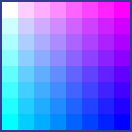
\includegraphics[width=0.9\linewidth]{figures/gradient.png}
    \caption{Gradient model}\label{fig:gradient}
\end{wrapfigure}
Code available in \cref{code:drawcon}.

As the most complex module written for this project, this module controls all graphical elements on the screen. 
It takes as input coordinates for the current drawing pixel and player, and outputs the colour of the pixel 
to be drawn. 

Subsequent sections (\ref{sec:colourpicker} and \ref{sec:colorgrid}) rely on a specific 
set of colours defined as a colour space, which is a 64-index array of 12-bit colour values.  
Following the progression that can be seen in \cref{fig:gradient},
the top left corner starts with a colour value of \lstinline|0xFFF| (white) and reduces 
by 2 in green horizontally (to magenta, \lstinline|0xF0F|) 
and by 2 in red vertically (to cyan, \lstinline|0x0FF|).
The leaves the bottom right most value as all blue (\lstinline|0x00F|).
This is encoded sequentially, with a snippet of the corner values of \cref{fig:gradient} 
shown in \cref{table:colourspace}.
\begin{table}[H]
    \centering
\begin{tabular}{c|ccl}
    Array index & Hexadecimal value & \multicolumn{2}{c}{Colour} \\
    \hline
    0           & \lstinline|0xFFF| & White     & \fcolorbox{black}{white}{\rule{0pt}{4pt}\rule{4pt}{0pt}} \\
    7           & \lstinline|0xF0F| & Magenta   & \fcolorbox{black}{hMagenta}{\rule{0pt}{4pt}\rule{4pt}{0pt}} \\
    56          & \lstinline|0xF0F| & Cyan      & \fcolorbox{black}{hCyan}{\rule{0pt}{4pt}\rule{4pt}{0pt}} \\
    63          & \lstinline|0xF0F| & Blue      & \fcolorbox{black}{hBlue}{\rule{0pt}{4pt}\rule{4pt}{0pt}} \\
\end{tabular}
\caption{\lstinline|colourspace| encoding}\label{table:colourspace}
\end{table}
Generation of the colour space occurs in a FOR loop, using the subtraction of \lstinline|0x020|
from \lstinline|0xFFF|\footnote{
    Lines 66-73 of \lstinline|draw_controller|. Details of implementation can be found in \cref{sec:test}.
}.

Subsequently, the elements to appear on-screen are drawn in hierarchical order. Order is determined 
by a conditional tree that evaluates when the coordinates of the pixel to be drawn are within the 
space defined for the element. The following snippet illustrates this idea, where the banner colour is 
drawn at the top of the screen, otherwise the background colour is drawn.
\begin{lstlisting}[language=Verilog]
    if (y_coord < BANNER_HEIGHT) begin
        pixel <= COL_BANNER;
    end else begin
        pixel <= COL_BACKGROUND;
    end
\end{lstlisting}

The following elements are drawn in order of hierarchy:
\begin{enumerate}
    \item ID sprite
    \item Banner
    \item Title sprite
    \item Screen border
    \item Player reticle sprite
    \item Gradient colour picker
    \item Picker selection area border
    \item Picker border
    \item Grid background
\end{enumerate}

\subsubsection{sprite\_reticle}\label{sec:sprite}
\begin{wrapfigure}[11]{R}{0.2\linewidth}    
    % \vspace{-10pt}
    \centering
    \begin{subfigure}[t]{\linewidth}
        \centering
        
\includegraphics[height=1.5cm,width=\linewidth,keepaspectratio]{figures/reticle_graphical.png}
        \caption{Intended appearance}\label{fig:spriteorig}
    \end{subfigure}    
    \vskip\baselineskip
    \begin{subfigure}[b]{\linewidth}
        \centering
        
\includegraphics[height=1.5cm,width=\linewidth,keepaspectratio]{figures/reticle_4.png}
        \caption{Encoded sprite}\label{fig:spriteencoded}
    \end{subfigure}
    \caption{Player sprites}
\end{wrapfigure}
The `player' sprite appears as a controllable reticle intended to point at the colour selected. 
The sprite was drawn in Microsoft Paint and 
converted from its base format (.bmp) to space delimited memory encoding (.coe) that 
can be used by Xilinx's block memory generator IP to write the sprite into ROM. 

Due to what is most likely issues with reading the sprite from memory, the image has been 
adjusted from \cref{fig:spriteorig} to \cref{fig:spriteencoded} to account for `wrapping'
that appears to occur. 

As a controllable object, additional complications are introduced as the sprite moves or 
generally interacts with the drawing logic. A pixel to be written from memory is skipped, 
leading to the appearance of `scrolling'. This is fixed by ensuring the first address 
from ROM is to be written after either the last address has been reached, or the 
current drawing coordinates (\lstinline|x_coord| and \lstinline|y_coord|) coincide with 
the current position of the sprite (\lstinline|player_pos_x| and \lstinline|player_pos_y|,
indicating the top left corner)\footnote{
    Lines 110-112 of \lstinline|draw_controller|.
}.

A final feature of the sprite is the red (\lstinline|0xF00|) pixels in the centre is 
used to determine the colour `selected'. When drawing the sprite, if the pixel being drawn is 
a red pixel, the pointer returned by \lstinline|gradient_pointer| from \lstinline|colour_picker|\footnote{
    \Cref{sec:colourpicker}.
} 
is recorded into \lstinline|selected_pointer| and the colour value held in \lstinline|col_selected|
in order to change the control area border colour. A similar technique is used to provide `transparency'
for the white portions of the sprite, simply by overriding the pixel colour 
with \lstinline|colourspace[gradient_pointer]|\footnote{
    Lines 114-121 of \lstinline|draw_controller|.
}.

\subsubsection{sprite\_title}
\begin{wrapfigure}[5]{R}{0.25\linewidth}
    \vspace{-30pt}
    \centering
    
\includegraphics[width=\linewidth]{figures/flood.png}
    \caption{Title sprite}
\end{wrapfigure}
A sprite for the title was created in Adobe Photoshop owing to its increased complexity in detail. 
The background colours were selected to fit seamlessly with the top banner of the game. 

It was rendered into the game from a ROM similar to the player sprite.

\subsubsection{sprite\_title}
Produces the ID values 2008503 and 1922268 in the top left corner. 

\subsubsection{colour\_picker}\label{sec:colourpicker}

Code available in \cref{code:colourpicker}.

This module creates the central colour selection region for the player, outputting 
a pointer for current pixel to be drawn.  

The initial idea was to create the selection colour space as a sprite, leading 
to the creation of \cref{fig:gradient} in Adobe Illustrator to be imported as a ROM. 
The sprite approach was changed as it consumes a large amount of memory\footnote{
    The first version with 256 16$\times$16 pixel cells required more memory than was available on the FPGA. 
}. 
A programmatic approach, using a FOR loop is used instead\footnote{
    Lines 35-41.
}. In this case, the 8$\times$8 grid is generated from a nested FOR loop; the 
outer loop specifies the height of the grid cells and the inner loop the width 
of the cell. The colour is then selected by a sequential counter 
pointing to \lstinline|colourspace|.

\subsubsection{colour\_grid}\label{sec:colorgrid}
Code available in \cref{code:colourgrid}.

This module works similar to \lstinline|colour_picker| 
in producing a grid from a nested FOR loop,
however it has to deal with the extra complexity 
of dynamically updating the colour of its cells.
This leads to some artefacts appearing as this logic 
interacts with the display adapter. The general logic of the game in terms of 
`flooding' is handled in this module. It receives the current colour pointer 
as in input and outputs a pointer for the colour of the current background 
pixel. 

Two 16$\times$16 2D arrays are used in this module\footnote{
    The file type was changed to SystemVerilog as multidimensional and unpacked arrays are not supported by Verilog. 
}: 
\begin{itemize}
    \item \lstinline|connected_array| -- Holds a value to describe the state of the cell.
    \begin{description}[align=left, labelwidth=0.5cm,labelindent=0.5cm]
        \item[2] The cell is `connected' and changes colour with the selection from \lstinline|colour_picker|.
        \item[1] The cell is adjacent to a `connected' cell, and needs to be checked if it matches the selection.  
        \item[0] The cell is in its default state. 
    \end{description}
    \item \lstinline|pointer_array| -- Holds the pointer to the colour for the cell. Starts `randomised'\footnote{
        \Cref{sec:randomisation}.
    }.
\end{itemize}

Every clock cycle, a single cell is analysed, with the entire grid checked over a million times in a single 
game frame. The incremental order is horizontally, then vertically. 
If the cell is adjacent (value \lstinline|1|), the colour is checked. If matched, the colour of the cell is updated 
to the currently selected colour (via \lstinline|pointer_array|), its \lstinline|connected_array| value updated to \lstinline|2|,
and each cell adjacent is updated to have a value of \lstinline|1| if currently \lstinline|0|. 
Otherwise, if the value is \lstinline|2|, the colour is simply updated\footnote{
    Lines 548-576.
}. 

\subsection{Unimplemented features}
\subsubsection{FOR loops}
In some instances, logic that had been hardcoded 
was successfully converted into a much easier to read 
and maintainable FOR loop. However, this is not the case in every instance. While the 
creation of the colour space in \lstinline|draw_controller|\footnote{
    \Cref{sec:drawcon}.
} was successfully converted, the same cannot be said for the value assignments 
to \lstinline|connected_array| in \lstinline|colour_grid|. The result, in the 
instances adjacency worked, appeared to match cells somewhat randomly 
or led to some cells failing to change colour. 

\subsubsection{Difficulty modes}
Different levels of gameplay difficulty, where the user selects an option 
that dictates the grid size (i.e. 8\textsuperscript{2} rather 
than 16\textsuperscript{2} - the current default) would have been implemented 
leveraging the dynamic nature of the grid generation if handled in a loop. 
In that case, the loop would be built into a conditional, where the 
selected grid size would inform the variables used to define each cell's 
width and height. Even the number of colours could be adjusted similarly
to lower the difficulty in discerning colours. 

\subsubsection{Randomisation}\label{sec:randomisation}
The grid was intended to be generated randomly for each game. 
Generating a string of random numbers is possible with a Linear-Feedback Shift Register (LFSR),
which produces a deterministic string of random numbers. The sequence is dependent on the initial 
input (seed), which itself would require true random generation in some manner. 
A possibility for this is to take a reading from the board temperature sensor. 

\subsubsection{Timer and completion}
The idea of `filling the grid as quickly as possible' falters at the point 
where the game lacks a timer for the user to see how quickly they have completed the board. 
\lstinline|clock_gen| would need to output a clock for seconds, incrementing a counter 
on every positive edge. Then, the program can
read from a numeral sprite map to render digits on screen that show the current 
decimal value of the counter.

Completion can be determined by summing \lstinline|connected_array|. A cell is matched 
when its value is \lstinline|2|. For a 256 cell array, if the sum equals 512, 
the game is finished. Extending this idea further allows showing the current 
percentage of completion. 


\section{Testing and verification process}\label{sec:test}
Testing designs before compiling them becomes ever more important as complexity scales. 
In the later stages of the project, a single compilation could take as much as ten minutes, 
highly restricting iterative testing methodologies like divide and conquer\footnote{
    A methodology where debugging statements are printed to console to narrow down the source of a problem.
    Highly reliant on running many test suites in quick succession. 
}. Therefore, the importance of testing via simulations is emphasised. 

To illustrate this process, an example will be outlined. Following an agile-like development methodology 
for this project prioritised producing functional code as quickly as possible. 
For static but repeatable elements, this means a large amount of hardcoded software, 
making the code unwieldy and increasing the difficulty maintaining the codebase.
To improve this, the logic can be synthesised from a FOR loop instead. 

\subsection{The hardcode}
\begin{lstlisting}
initial begin
    colourspace[0] <= 12'hfff;
    colourspace[1] <= 12'hfdf;
    colourspace[2] <= 12'hfbf;
    ... 
    colourspace[7] <= 12'f1f;
    colourspace[8] <= 12'dff;
    ... 
    colourspace[63] <= 12'h11f;
end
\end{lstlisting}
This was generated from the following Python script (modified slightly for clarity):
\begin{lstlisting}[language=Python]
    r = 15
    g = 15
    b = 15
    for count in range(0,64):
        print(f"colorspace[{count}] <= 12'h{r:x}{g:x}{b:x};")
        g = g - 2
        if(g < 0):
            r = r - 2
            g = 15
\end{lstlisting}

\subsection{Rewrite in Verilog}
The hardcoded logic can be synthesised from a FOR loop, written in Verilog directly in this case.
This is almost a direct translation from the Python script to Verilog, however there are a number of differences. 
Since the code does not need to be printed to be copied, that stage is omitted entirely. Instead, the assignment of the 
colour to \lstinline|colourspace| is made directly through an intermediary variable \lstinline|tcol|, 
which is made of the \lstinline|r|, \lstinline|g|, and \lstinline|b| bitshifted to their respective places.
\begin{lstlisting}[language=Verilog]
for(i=0;i<64;i=i+1)begin
    tcol = r<<8;
    tcol = tcol + g<<4;
    tcol = tcol + b;
    colourspace[i] = tcol;
    g = g - 2;
    if(g < 1) begin
        r = r - 2;
        g = 4'hf;
    end
end
\end{lstlisting}
This can then be run in a test bench to see the resultant values of
\lstinline|tcol|, \lstinline|r|, \lstinline|g|, \lstinline|b|, and \lstinline|colourspace|.
\begin{figure}[H]
    \centering
    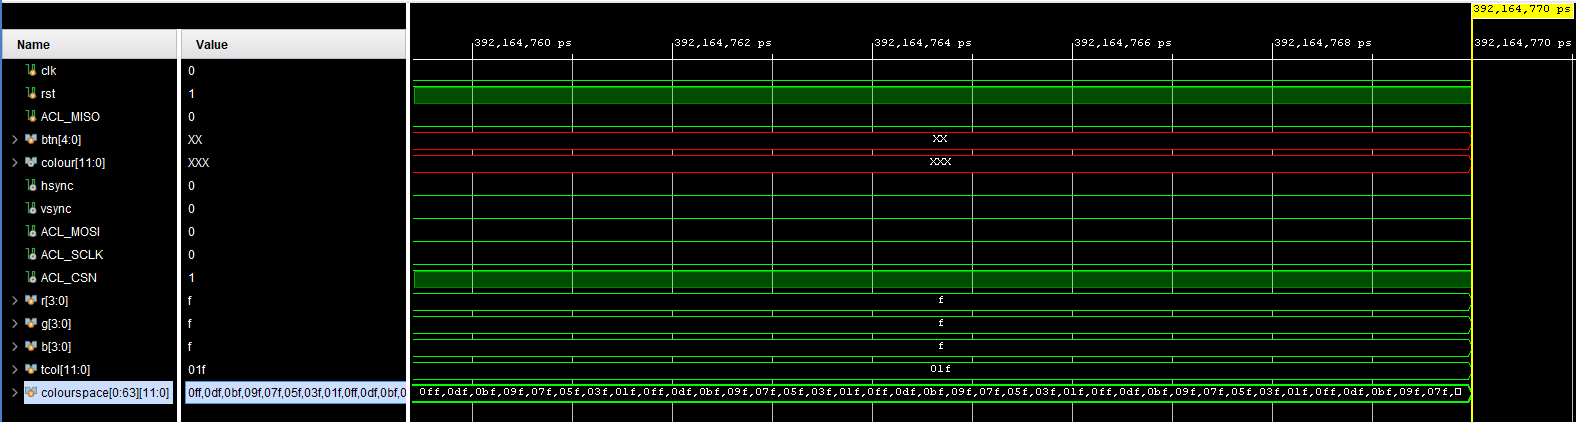
\includegraphics[width=\textwidth]{figures/tb/1.png}
\end{figure}
The resulting colour values are not quite correct, with the red value stuck at 0.

\begin{minipage}{0.475\linewidth}
\begin{lstlisting}[language=Verilog]
for(i=0;i<64;i=i+1)begin
    colourspace[i] = r<<8 + g<<4 + b;
    g = g - 4'h2;
    if(g < 4'h1) begin
        r = r - 4'h2;
        g = 4'hf;
    end
end    
\end{lstlisting}
\end{minipage}\hfill
\begin{minipage}{0.5\linewidth}
    \centering
    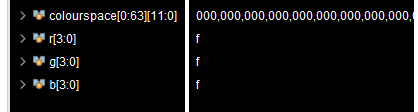
\includegraphics[width=\linewidth]{figures/tb/2.png}
\end{minipage}
This attempts to perform the bit-shift in a single line, however the end result is all 0.
The intermediary variable is necessary. 

\begin{minipage}{0.475\linewidth}
\begin{lstlisting}[language=Verilog]
for(i=0;i<64;i=i+1)begin
    tcol = tcol + g<<4;
    tcol = tcol + b;
    colourspace[i] = tcol;
    g = g - 4'h2;
    if(g < 4'h1) begin
        r = r - 4'h2;
        g = 4'hf;
    end
end
\end{lstlisting}
\end{minipage}\hfill
\begin{minipage}{0.5\linewidth}
    \centering
    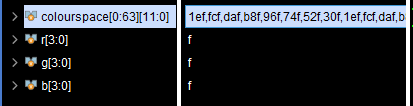
\includegraphics[width=\linewidth]{figures/tb/3.png}
\end{minipage}
This indicates the red bit-shift is always returning 0 and non-functional. 
The gradient produced is also not what is intended. It may be better to move 
to subtracting a constant value. 

\begin{minipage}{0.475\linewidth}
\begin{lstlisting}[language=Verilog]
for(i=0;i<64;i=i+1)begin
    colourspace[i] = tcol;
    tcol = tcol - 12'h020;
    if(tcol[7:4] < 4'h1) begin
        tcol = tcol - 12'h200;
    end
end
\end{lstlisting}
\end{minipage}\hfill
\begin{minipage}{0.5\linewidth}
    \centering
    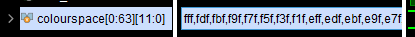
\includegraphics[width=\linewidth]{figures/tb/4.png}
\end{minipage}
This subtractive method appears better, however the aim is to drop the red value by two, whereas here it only drops by one.
The loop in an \lstinline|initial| block does not appear to be synthesised correctly for actual implementation, resulting
in a black screen.

\begin{minipage}{0.475\linewidth}
\begin{lstlisting}[language=Verilog]
for(i=0;i<64;i=i+1)begin
    colourspace[i] = tcol;
    tcol = tcol - 12'h020;
    if(tcol[7:4] < 4'h1) begin
        tcol = tcol - 12'h500;
    end
end 
\end{lstlisting}
\end{minipage}\hfill
\begin{minipage}{0.5\linewidth}
    \centering
    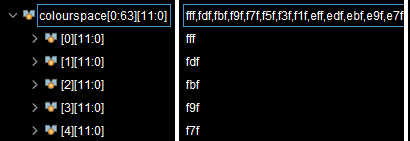
\includegraphics[width=0.9\linewidth]{figures/tb/5.png}
\end{minipage}
The code was moved to an \lstinline|always| block to allow it to be synthesised to the display correctly. 
Furthermore, the reduction was increased. The test bench shows the value stay the same - the 
IF statement is not evaluating true since \lstinline|tcol[7:4]| will move from 1 to F. 

\begin{minipage}{0.475\linewidth}
\begin{lstlisting}[language=Verilog]
for(i=0;i<64;i=i+1)begin
    colourspace[i] = tcol;
    tcol = tcol - 12'h020;
    if(tcol[7:4] == 4'hf) begin
        tcol = tcol - 12'h100;
    end
end 
\end{lstlisting}
\end{minipage}\hfill
\begin{minipage}{0.5\linewidth}
    \centering
    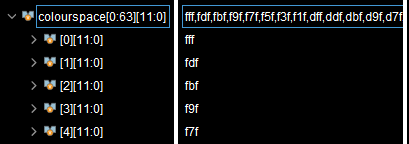
\includegraphics[width=0.9\linewidth]{figures/tb/6.png}
\end{minipage}
The values are now reducing in the correct progression. 

\section{Conclusion}

\subsection{Evaluation}
The designed game will be evaluated against the criteria. 
\paragraph{User control}
The user takes control of a reticle to select a colour, which is controllable
by tilting the board in the desired movement direction. The sprite is 
bounded within the selection area. 
\paragraph{Object interactions} 
The game progresses by clearing the screen by progressively selecting colours. 
The grid items need to effectively interact with each other in order to determine 
adjacency and when a grid has been matched to the selected colour. However, 
some visual artefacts may occur. 
The player sprite also interacts with the selection grid underneath to select a 
colour and assumes the characteristics of transparency. 
\paragraph{Info bar}
An info bar is drawn from the graphics controller as a banner at the topmost
hierarchical layer, and includes sprites for the game title and IDs. 
\paragraph{Extra hardware}
The game makes use of the in-built accelerometer, available on the SPI interface,
in order to control player movement. It also displays the game title on the 7-segment display. 
\paragraph{Sprites}
The game makes use of 3 sprites, one for the player, title, and IDs. 
There are some issues with the player sprite appearance, where the sprite is shifted somewhat. 
However, these have been mitigated by adjusting the sprite ROM to negate this effect.

\subsection{Reflection} 

\paragraph{Colour blindness support}
The game in its current form is not supportive of most forms of colour vision deficiency, with the likely exception of 
tritanopia and tritanomoly. Support can be increased by adjusting the colour space used, i.e. using a 
Cividis or Viridis colour space \cite{Nunez2018}, or allowing different colour selections by the player.

Support for achromatopsia may prove difficult while retaining game flow and simplicity. One possible solution is 
to use symbolic elements on cells, and improve the animation between cells to indicate matching. This would, however, 
require a significant redesign of the game logic. 

\subsubsection{Player comments}
During player testing, a notable complaint that cropped up was the difficulty of matching a colour,
with the controls feeling `slippery' and `imprecise'. 
This issue can be broken down into two parts - difficulty in identifying the colour to match, and moving to that colour. 
\paragraph{Identification} With the 64 colour selection, differentiating tones in the same quadrant 
can prove difficult. Colour definition can be improved with a greater display resolution, perhaps by moving 
to a more up-to-date display standard, although this would require the requisite adapter to be available on the board. 
\paragraph{Movement} Movement is altogether both too responsive and not responsive enough. This makes fine adjustments
difficult and overshoots frequent. Overshoots can be improved with the current accelerometer implementation 
by compressing the responsive range to cover half the rotation it does currently. In other words, rather than a complete 
half turn returning 16 (the greatest value), only a quarter turn is needed, with every second value skipped. The 
downside is that fine adjustments will be made more difficult. A complete reimplementation of the accelerometer 
will be needed to return data in finer intervals to combat this. 

\subsubsection{General comments}
The development process for the game was not smooth. Debugging, especially for graphical glitches or 
player interactions, proved particularly difficult to manage. 
This is due to how they cannot be observed easily within test benches. Some issues also 
do not appear to be problematic in test benches, whereas fail to render in actual implementation. 
The final implementation also suffers some logical glitches, where a cell remains unmatched. Overall,
the game functions fairly well otherwise. 

\nocite{digilentmanual}

\printbibliography


\clearpage
% \begin{landscape}
\begin{appendices}
\pagenumbering{roman}

% \lstinputlisting[language=Matlab, caption={Power meter graphing script},label=script:powermeter]{../../Tests/power meter/powermeter.m}
% \clearpage

\section{Code}

\subsection{Main files}
\lstinputlisting[language=Verilog, caption={game\_top.v},label=code:gametop]{./example code/game_top.v}
\clearpage
\lstinputlisting[language=Verilog, caption={clock\_gen.v},label=code:clockgen]{./example code/clock_gen.v}
\clearpage

\subsection{Graphics}
\lstinputlisting[language=Verilog, caption={drawcon.v},label=code:drawcon]{./example code/drawcon.v}
\clearpage
\lstinputlisting[language=Verilog, caption={colour\_picker.v},label=code:colourpicker]{./example code/colour_picker.v}
\clearpage
\lstinputlisting[language=Verilog, caption={colour\_grid\_i.sv},label=code:colourgrid]{./example code/colour_grid_i.sv}
\clearpage

\subsection{Display}
\lstinputlisting[language=Verilog, caption={vga\_out.v},label=code:vga]{./example code/vga_out.v}
\clearpage

\subsection{Seven-segment display}
\lstinputlisting[language=Verilog, caption={seginterface.v},label=code:seginterface]{./example code/seginterface.v}
\clearpage
\lstinputlisting[language=Verilog, caption={sevenseg.v},label=code:sevenseg]{./example code/sevenseg.v}
\clearpage

\end{appendices}
% \end{landscape}

\end{document}